\chapter{Federated Edge}


Figure~\ref{fig:edge} illustrates the overview of a deployment of distributing data processing tasks to the edge of the IoT.
Similarly to a typical deployment of an IoT system, in the perceived layer, the low-end devices (e.g., sensors, actuators) can be deployed across several sites in different locations (e.g., houses or weather stations).
The devices in the same site can be connected to a gateway device that gives access to the produced data.
In IoT cloud-based systems~\cite{Petrolo:2014}, all the sensory data is pushed to cloud or a centralised node on which data integrating and data accessing take place.
In contrast of the deployments, we aim to push these tasks away from a centralised node by leveraging the advance computing resources of the gateway devices.
Therefore, we adopt mediator-based architecture~\cite{Garcia-molina:1995} in our model.
Gateway devices are attached a software component thus becoming mediators~\cite{Wiederhold:1992} for data integrating and accessing.
The mediator will allow physical data produced from the low-end devices to be wrapped into a common data model, and then to be stored on the gateways node.
Queries can be issued from a gateway, and can be federated to other connected gateways. 
The federation enables data to be accessed in the same manner as a centralised system. 

\begin{figure}[h!]
\centering
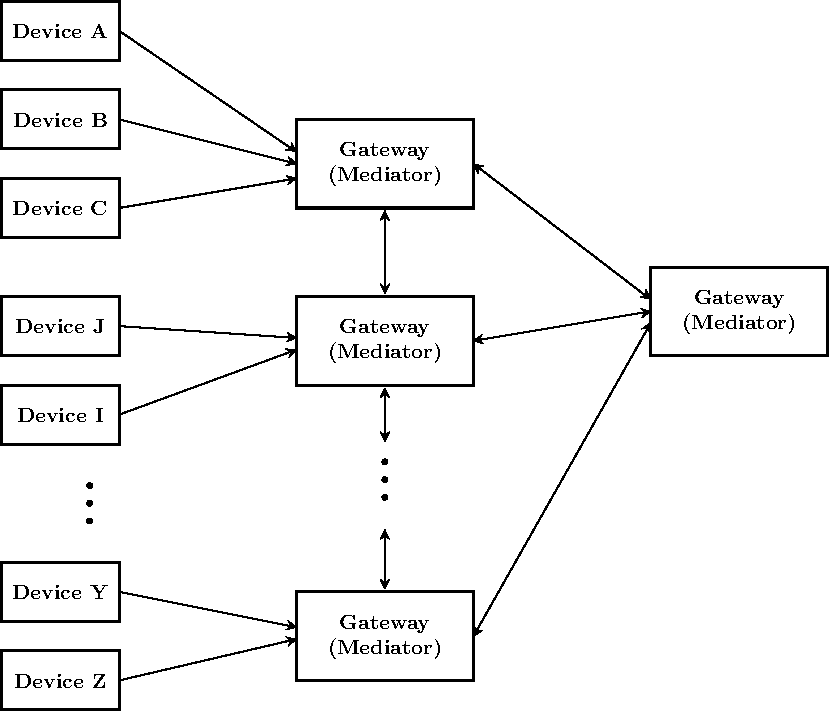
\includegraphics[width=0.35\textwidth]{c7/edge.pdf}
\caption{Overview of distributed architecture}
\label{fig:edge}
\end{figure}

In order to enable seamless integration across all the system, Linked Data technologies can be considered.
Since the high-end devices have enough computational resources, RDF engines can be brought to the gateway nodes to create such mediators.
Physical data from low-end devices can be wrapped into RDF data and can be locally stored using an RDF storage.
The federation mechanism of federated SPARQL queries can be also leveraged.
Simple data model of SPARQL federation such as RDF serialisation or SPARQL result can be used for information exchange between mediators.

\section{Gateway descriptor}

Semantic source selection: source can be select by it attributes.
why this is important. 

There are many approaches for source selection. Why do we need discovery???
each gateway is an endpoint - we can send ask query for each node for discovering.
We can use DHT to index source. From the subquery $\to$ select relevant source set.





In the IoT context, the sources are the \textit{"things"} which provide specific data, services.
Consumers cannot be asked to know the specific sources to navigate the federated queries.
Therefore, supporting automatic source discovery is one of major requirements for the mediators.
They should understand the meta-information of the connected things in the system, hence, 
query can be delivered to the mediators that things are connected.









A Thing in the system can be described using \textit{Thing Description (TD)}~\footnote{https://www.w3.org/TR/wot-thing-description/} framework. 
TD provides the syntax to describe the meta-information of thing (e.g., name of Thing, type of Thing), 
the interaction patterns (e.g., readable/writeable data on Thing, 
actions that can be triggered on Thing, events that are notified by Thing) and communication metadata.
TD can be represented using JSON-LD which is extremely lightweight and beneficial for constrained devices.
Listing~\ref{lst:TDexample} shows a sample TD of a temperature sensor named "MyTemperatureThing".
The sensor is serving a temperature reading as a Property.
The reading is accessible over CoAp protocol at the endpoint "coaps://mylamp.example.com:5683/" and is returned within a JSON-LD structure.


\begin{lstlisting}[language=sparql,
  				   captionpos=b,
                   label={lst:TDexample},
                   caption={SPARQL}]       
PREFIX sosa:<http://www.w3.org/ns/sosa/>                   
PREFIX ex:<http://example.org/featureOfInterest/>                   

SELECT ?tempValue ?windValue
{
 ?windObservation a sosa:Observation. 
 ?windObservation sosa:hasFeatureOfInterest ex:Wind.
 ?windObservation sosa:hasSimpleResult ?windValue.
 ?windObservation sosa:resultTime ?time.
 ?tempObservation a sosa:Observation.
 ?tempObservation sosa:hasFeatureOfInterest ex:Temperature.
 ?tempObservation sosa:hasSimpleResult ?tempValue.
 ?tempObservation sosa:resultTime ?time.
}
\end{lstlisting}



\begin{lstlisting}[language=sparql,
  				   captionpos=b,
                   label={lst:TDexample},
                   caption={Federated SPARQL}]
PREFIX sosa:<http://www.w3.org/ns/sosa/>                   
PREFIX ex:<http://example.org/featureOfInterest/>  

SELECT ?tempValue ?windValue {
SERVICE <ex:gatewayA> {
 ?windObservation a sosa:Observation. 
 ?windObservation sosa:hasFeatureOfInterest ex:Wind.
 ?windObservation sosa:hasSimpleResult ?windValue.
 ?windObservation sosa:resultTime ?time. }
SERVICE <ex:gatewayA> {
 ?tempObservation a sosa:Observation.
 ?tempObservation sosa:hasFeatureOfInterest ex:Temperature.
 ?tempObservation sosa:hasSimpleResult ?tempValue.
 ?tempObservation sosa:resultTime ?time.}
}
\end{lstlisting}

\begin{lstlisting}[language=sparql,
  				   captionpos=b,
                   label={lst:TDexample},
                   caption={Federated SPARQL}]
PREFIX sosa:<http://www.w3.org/ns/sosa/>                   
PREFIX ex:<http://example.org/featureOfInterest/>  

SELECT ?temp {
 ex:DeviceA ssn:hasSubSystem ?sensor
 ?sensor a sosa:Sensor.
 ?sensor sosa:madeObjervation ?observation.
 ?observation ex:hasValue ?temp.
}
\end{lstlisting}


\section{Source Selection}


\begin{lstlisting}[language=sparql,
  				   captionpos=b,
                   label={lst:TDexample},
                   caption={Federated SPARQL}]
PREFIX sosa:<http://www.w3.org/ns/sosa/>                   
PREFIX ex:<http://example.org/featureOfInterest/>  

SELECT ?tempValue {
 ?gateway ssn:Subsystem ?sensor
 ?sensor  a ssn:Sensor.
 ?sensor  a ex:Temperature.
 
 Service <?gateway>
 {
  ?tempObservation a sosa:Observation.
  ?tempObservation sosa:hasFeatureOfInterest ex:Temp.
  ?tempObservation sosa:hasSimpleResult ?tempValue.
  ?tempObservation sosa:resultTime ?time.
 }
}
\end{lstlisting}



The federated search consists of organizing service information in a set of information repositories and managing them to perform the service discovery tasks.
For example: If we want to query temperature data using sparql query.
The federator has to discover which mediator connects to temperature data.


\begin{lstlisting}[language=sparql,
  				   captionpos=b,
                   label={lst:TDexample},
                   caption={Simple TD example describing a mediator}]
SELECT ?temphref {
  ?device td:interaction ?property
  ?property a td:Property.
  ?property a iot:Temperature.
  ?property td:form ?form.
  ?form td:mediaType "application/jsonld"
  ?form td:href ?temphref.
}
\end{lstlisting}


Search criteria can be considered as the queries that trigger the discovery process which is expected to end up providing a ranked set of matching thing descriptions to the issuer. 
In case a query language, e.g., SPARQL is used for expressing semantic search criteria, all involved actors should at least know about its protocol, i.e., communications established between an issuer and a directory must implement the corresponding query language protocol. 
A high level of expressiveness of the query language used will likely broaden the possibilities
for discovery requests, e.g., features for filtering and aggregating.

Mediator:
Not exact match 
Reasoning $\to$ match
SPARQL Update $\to$ 


\begin{lstlisting}[language=sparql,
  				   captionpos=b,
                   label={lst:TDexample},
                   caption={Simple TD example describing a mediator}]
SELECT ?temphref {
  ?device td:interaction ?property
  ?property a td:Property.
  ?property a iot:Temperature.
  ?property td:form ?form.
  ?form td:mediaType "application/jsonld"
  ?form td:href ?temphref.
}
\end{lstlisting}










